\documentclass[a4paper,10pt]{article}

% Wider pages.
\usepackage[a4paper]{geometry}

% Language.
\usepackage[english]{babel}

% Allows the use of \subtitle{...}.
\usepackage{titling}
\newcommand{\subtitle}[1]{%
  \posttitle{%
    \par\end{center}
    \begin{center}\large#1\end{center}
    \vskip0.5em}%
}

% Allows the use of \includegraphics{...}.
\usepackage{graphicx,subfigure}

% Allows the use of \url{...}.
\usepackage{url}

% Seperate paragraphs by an empty line and removes indentation.
\usepackage[parfill]{parskip}

\begin{document}

%%%%%%%%%%%%%%%%%%%%%%%%%%%%%%%%%%%%%%%%%%%%%%%%%%%%%%%%%%%%%%%%%%%%%%%%%%%%%%%
% TTITLEPAGE
%%%%%%%%%%%%%%%%%%%%%%%%%%%%%%%%%%%%%%%%%%%%%%%%%%%%%%%%%%%%%%%%%%%%%%%%%%%%%%%
\title{Evolving ice skating behavior with a Nao robot in a simulated environment using HyperNEAT}

\author{Bas Bootsma (0719080) \and Roland Meertens (3009653) \and Tom de Ruijter (3016269)}

\date{January 22, 2012}

\maketitle

%%%%%%%%%%%%%%%%%%%%%%%%%%%%%%%%%%%%%%%%%%%%%%%%%%%%%%%%%%%%%%%%%%%%%%%%%%%%%%%
% INTRODUCTION
%%%%%%%%%%%%%%%%%%%%%%%%%%%%%%%%%%%%%%%%%%%%%%%%%%%%%%%%%%%%%%%%%%%%%%%%%%%%%%%
\section{Introduction}
...

Literature background...

In section \ref{sec:initial-experimental-setup} \emph{Initial Experimental Setup} most of the details of the project will be explained and our .... In section ...

%%%%%%%%%%%%%%%%%%%%%%%%%%%%%%%%%%%%%%%%%%%%%%%%%%%%%%%%%%%%%%%%%%%%%%%%%%%%%%%
% INITIAL EXPERIMENTAL SETUP
%%%%%%%%%%%%%%%%%%%%%%%%%%%%%%%%%%%%%%%%%%%%%%%%%%%%%%%%%%%%%%%%%%%%%%%%%%%%%%%
\section{Initial Experimental Setup}
\label{sec:initial-experimental-setup}


\subsection{NEAT}
NeuroEvolution of Augmenting Topologies (NEAT) technique developed Ken O. Stanley in 2002, which makes use of genetic algorithms for evolving artificial neural networks \cite{wikipedia:neat}. The technique both alters the weights and the structure (topologies) of the network to find a balance between the fitness and the diversity of the solutions. NEAT has several properties which make it an interesting technique.

\begin{itemize}
	\item \textbf{Complexifying}: Complexifying is the incremental increase of complexity over time. This means that NEAT starts out with simple topologies and gradually increases complexity over generations.
	\item \textbf{Speciation}: With speciation topologies which are similar are grouped together in niches. This protects for example new topologies, which generaly have worse fitness when compared to already existing topologies, thus allowing the new topologies evolve in a protected niche instead of immediatly discarding them.
	\item \textbf{Historical marking}: Each gene is assigned a unique historical marker which allows later generations to track origin of their genes.  
\end{itemize}

\subsection{HyperNEAT}
HyperNEAT is the successor of NEAT and provides several extra properties which we believe are beneficial for generating ice skating behavior.

\begin{itemize}
	\item \textbf{Geometric relationships}: HyperNEAT is aware of the geometric relationships of the input. In our case this means that it not only knows the different joints, but also the relationships between the joints. For example, it might be able to exploit the relationship between the ankle and knee joint by posing extra restrictions to prevent the Nao robot from falling over.
	\item \textbf{Symmetrical and recurrent patterns}: HyperNEAT is able to find symmetrical and recurrent patterns. In our case this is important, since ice skating behavior contains symmetrical and recurrent elements, which we hope HyperNEAT is able to find.
\end{itemize}


%%%%%%%%%%%%%%%%%%%%%%%%%%%%%%%%%%%%%%%%%%%%%%%%%%%%%%%%%%%%%%%%%%%%%%%%%%%%%%%
% HYPOTHETICAL EXPERIMENTAL SETUP
%%%%%%%%%%%%%%%%%%%%%%%%%%%%%%%%%%%%%%%%%%%%%%%%%%%%%%%%%%%%%%%%%%%%%%%%%%%%%%%
\section{Hypothetical Experimental Setup}
\label{sec:hypothetical-experimental-setup}
In the previous section we have explained the major details of our project and we also have explained how we did not get HyperNEAT to work successfully. In the case that we did got HyperNEAT working successfully we would have liked to perform several experiments. In the following sections the hypothetical setup, the experiments and the related settings of the HyperNEAT algorithm.

\subsection{Setup}
\label{sec:setup}
As we already explained we would have wanted to use a different approach, namely using a direct feedback loop from the simulator to the HyperNEAT algorithm. This means that for each time step $t$ the current joint values of the robot in the simulator are read and feed as input into the HyperNEAT algorithm which produces the joint values for time step $t + 1$. Trying to evolve a complete behaviour (i.e. a motion file) has deemed to prove too difficult. However the described approach allows for a more direct mapping between the evolving behavior and the HyperNEAT algorithm in which the problem can be solved in smaller steps. A similar approach was used in evolving a walking gait for a quadruped using generative enconding \cite{EvolvingCoordinatedQuadrupedQaitsWithTheHyperNEATGenerativeEncoding}. It is not yet possible to tell exactly how long the algorithm should run. However since we are evolving a behaviour one step at a time we can increase or decrease the time needed to find a suitable ice skating behaviour.

\subsection{Experiments}
In order to investige our research question, whether it is possible to learn ice skating behavior to a Nao robot in a simulated environment, we would have to perform several experiments. As we have already explained ice skating behaviour consists of two phases, namely the startup phase and the recurrent phase. Since we are primarely interested in the recurrent phase all the experiments focus on trying to evolve an behaviour which has the property of a recurrent motion. This means that any evolved behavior not only has to work for the duration in which the algorithm runs, but also for durations larger than what is being evolved for. It seems logical to make use of the scaling abilities of HyperNEAT to scale up in time. 

\subsubsection{Condition: With Initial Velocity}
For the baseline condition we are interested in the recurrent phase of an ice skating behavior. Therefor we want to investigate whether it is possible to evolve an ice skating behavior from a standing position with an initial velocity. This means that the Nao is in the initial position (i.e. all the joints are initially at 0) and a specific force has been applied to the robot which results in a certain velocity. Using this setup the algorithm can focus completely on the recurrent phase of ice skating behaviour.

\subsubsection{Condition: From Resting Position}
If the evolved behaviour from the condition with an initial velocity for the Nao robot, works out out well, we want to investigate whether it is possible to evolve a similar behaviour from a resting position. In this condition the initial position of the Nao robot is the same as the condition with the initial velocity except no velocity is given. This means that the algorithm has to evolve a behaviour for both phases. This condition will probably take much more computational time to 

In the case that both previous conditions produced no suitable ice skating motions there was also a different approach we could have taken. That is adding an already evolved behaviour to the popuplation. In this case there were two behaviours possible, namely a standard walking behaviour and a human ice skating behaviour. Even if both previous conditions did produce suitable ice skating motions it would still have been interesting to investigate whether adding such behaviours by default to the population would help to evolve a suitable ice skating behaviour.

\subsubsection{Condition: Walking Behaviour}
By default a walking behaviour is already provided by Webots containing the exact joint values at each time step. We could have used the motion file to train the algorithm with a fitness function based on how much the output differs from the already known joint values. After a certain number of generations or until the algorithm has perfectly learning the motion we could then save the network and when evolving any of the previous two behaviours already add it to the population. Putting an already evolved behaviour in the population could enhance the  

\subsubsection{Condition: Human Ice Skating Behaviour From a Kinect}
A similar procedure as with the walking behaviour can be done using data from a Kinect. Since a Kinect provides allmost the same joints as available in a Nao robot, it would have been possible to have a human perform some \emph{dry} ice skating in front of a Kinect. After some processing (i.e. removing unwanted joints) we could then feed this data to the algorithm and use the produced network in the same was as with the walking behaviour.

\subsection{HyperNEAT Settings}
For the hypothetical experiment setup we use Another HyperNEAT Implementation (hereafter called AHNI) by O. Coleman. Using a configuration file we are able to set certain properties of the algorithm. The most interesting ones will be discussed in the following sections.

\subsubsection{General}
HyperNEAT is set to run a certain amount of \emph{evolutions}. In each evolution a certain amount of \emph{generations} will be performed, which consist of evaluating the fitness of the current population and generating the next population. The default values of the number of evolutions and the number of generations are set at 100 and 50 respectively. We have no idea whether these settings would work and therefor a lot of experimenting is needed.

Another important property is the number of individuals in the population. By default this value is 10, which seems fair. However, it might be necessary to increase this value to allow for enough speciation, but this also increases the computational complexity. Thus keeping a fine balance between enough speciation and computation complexity is needed. Furthermore it is possible to use elitism for selecting when creating new generations. Since we think that evolving suitable ice skating behaviour takes a long time, keeping track of the best individuals seems a wise choice.

For all the experiments it is also important to make use of the scaling abilities of HyperNEAT. With scaling it is possible to take an already evolved network and scale it both horizontally and vertically without the need for extra training. However, in our case we are only interested in the vertical (in time) scaling, since both the number of inputs and outputs are fixed. In AHNI scaling always works in both directions, thus it might not even be possible to make use of this.

An important aspect of HyperNEAT is the fact that it is able to use spatial location while evolving. Since spatial location for a Nao robot matters, for example the right hip is attached to the right knee, the algorithm could use this information to find a suitable ice skating behaviour.

\subsubsection{Mutation}
HyperNEAT evolves topologies of neural networks. Therefor mutation involves adding, removing and changing of neurons, connections and weights. Ofcourse, no neurons can be added to or removed from the input and output layers, since those values are fixed. AHNI allows to adjust the rate at which the neurons, connects and weights are mutated. It is important to have enough mutation such that topologies can be formed to capture the complex ice skating behaviour. However, having too much mutation makes finding a suitable ice skating behaviour very difficult. Thus, a lot experimenting with the different values is necessary. 

\subsubsection{Topology}
The initial topology of the algorithm would consist of a single input and output player. They would both contain the same amount of neurons (i.e. equal to the amount of joints involved) and the network would be fully connected. The values of the weights would initially be random. Since each neuron is able to have its own activation function it is necessary to set the allowed activation functions. By default, these are the sigmoid, Gaussian, sine and absolute functions. At least the sigmoid and the sine functions would be necessary to evolve networks to allow for the recurrent phase of ice skating behaviour. However, other functions could also prove useful, thus experimenting with diffent activation functions seems necessary.

\subsection{Expected Results}
@TODO: ...


%%%%%%%%%%%%%%%%%%%%%%%%%%%%%%%%%%%%%%%%%%%%%%%%%%%%%%%%%%%%%%%%%%%%%%%%%%%%%%%
% PROOF OF CONCEPT
%%%%%%%%%%%%%%%%%%%%%%%%%%%%%%%%%%%%%%%%%%%%%%%%%%%%%%%%%%%%%%%%%%%%%%%%%%%%%%%
\section{Proof of Concept}
\label{sec:proof-of-concept}
As described in section \ref{sec:hypothetical-experimental-setup} HyperNEAT does not generate any suitable values. As a way of demonstrating that (except for the neuro evolution algorithm algorithm) our implemented setup works an alternative evolutionary algorithm is implemented. The fitness functions described in section \ref{sec:initial-experimental-setup} are implemented in Java, which brought the choice of our evolutionary algorithm to the easily usable and implementable Genetic Algorithms and Genetic Programming component (JGap). 

\begin{figure}[h!]
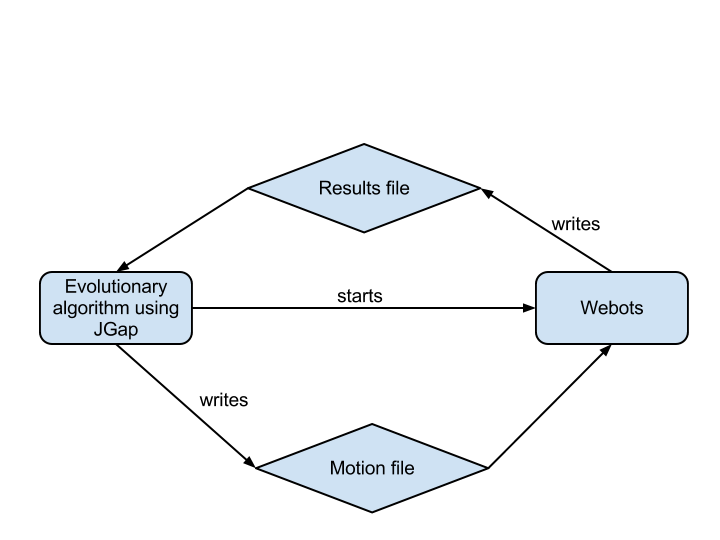
\includegraphics{images/jgapSetup}
\caption{Setup used for running our evolutionary algorithm}
\label{fig:jgapsetup}
\end{figure}

JGap is provided as a Java framework and provides basic genetic mechanisms that can be easily used to apply evolutionary principles to problem solutions \cite{jgap}. JGap is free of charge and can be downloaded at \url{http://jgap.sourceforge.net/}. 

As described in section \ref{sec:setup} the representation the motion of our Nao robot is represented as a two-dimensional array with double values. As JGap works with a genome consisting of an array of alleles consisting of double values a simple algorithm is written to converge the one-dimensional output of JGap into a two-dimensional array. 

During the generating of the next generation of chromosomes the existing chromosomes are crossed over. It is very probable that a chromosome generates a motion in which the first half is a very suitable motion, but leads to the Nao falling over halfway during this motion. This leads to our choice of the single-point crossover parameter which randomly selects a point to start the crossover. 

Continuously generating new generations of chromosomes by crossing over leads to a very small amount of alleles surviving and leads to sparsity of diversity in the population. Due to this a mutation parameter is introduced. The downside of mutation is that a mutated chromosome is more likely to introduce a “wrong” parameter at the start of a file. This makes mutation dangerous and leads to our choice of mutating only 1/12 of chromosomes. 

After each generation the chromosomes used in the next generation are selected. As there is not one definite motion the algorithm has to converge to even sub-optimal chromosomes have to survive. Our algorithm selects the best 90 percent of chromosomes each generation and uses these to generate the next generation. These chromosomes are manipulated, and the best chromosome is preserved to prevent it from dying after all manipulations. 

There are a lot of different motions that our Nao can perform to achieve a forwards motion. This means that even a motion that is not ideal is able to evolve into a motion that has a high fitness. With this in mind, ideally the population size is very large, as this gives more way to innovative solutions. Unfortunately the computation time of the fitness function is very large, as described in section \ref{sec:fitnessFunctions}. To speed up the simulation a population size of only 30 is chosen. 

As there is no clear goal that our Nao has to reach while moving forward and our algorithm is not able to run forever an amount of maximum generations is selected as termination condition. As there was not a lot of time to run our algorithm the termination condition taken was 200 generations. 


\section{Analysis of the results}
\label{sec:analysisOfTheResults}
\subsection{Arm moving}
\label{sec:resultsJGapArmMoving}
-> Graph-like thing that describes how the fitness improves over the different generations

During the running of the evolutionary algorithm with the arm moving fitness function no real milestones can be found. The algorithm starts with moving its arm randomly, and keeps selecting a better arm-raising motion every generation. 

Unfortunately our final chromosome still has values that are terribly off compared to the ideal values. Apart from this “problem” the final result looks like a very solid arm movement. The conclusion of our arm moving fitness function is that evolutionary algorithms are very capable of producing the simple movement of one joint. 

\subsection{Moving forwards for four seconds}
\label{sec:resultsJGapForwardsMoving}
-> Graph-like thing that describes how the fitness improves over the different generations

In the first five generations the evolved behaviours consist of our Nao performing some random movement which leads to a strange forwards motion. Starting from generation six the algorithm develops a rolling motion that ends at the four second mark. As our distance-measure point is the middle of our robot this makes a lot of sense. By performing a roll a little bit of extra distance is gained during the four seconds in which the motion is performed. Starting at iteration 120 a new behaviour emerges: sidewards \emph{shuffling}. This behaviour proves to be the best reachable behaviour in 200 generations as no better behaviour is found. 

Although our best chromosome after 200 generations is capable of traversing a large distance in four seconds it does not look like a very stable walking gait. Evolutionary algorithms thus are very capable of producing an advanced movement like this when they have enough time. The other conclusion is that the produced gait is not stable enough to use in a real robot, it thus is necessary to improve our fitness function. 

\subsection{Repeated motion for twelve seconds}
\label{sec:resultsJGapForwardsMovingTwelveSeconds}
-> Graph-like thing that describes how the fitness improves over the different generations

In the first five generations the evolved behaviours consist of our Nao performing some random movement leading to eventually falling on its back. In generation six our algorithm discovers that by turning around at the start of the motion it gains a little more distance (as the measure point for distance is the middle of our robot). In the same generation it starts to walk by using its arms as support (just like a gorilla). It also generates a motion that prevents the Nao from falling, consecutive generations improve the motion and keep preventing our Nao from tumbling over (except for generation 60).

Although our best chomosome after 200 iterations is capable of traversing a large distance in twelve seconds by repeating the four seconds long motion three times it unfortunately does not look like a very stable gait. Evolutionary algorithms thus are also very capable of producing an advanced repeated movement like this when they have enough time. Just like the fitness function of the four second long motion (in section \ref{sec:resultsJGapForwardsMoving} this motion is not stable enough to use in a real robot and our fitness function has to be improved. 

\subsection{Ice skating}
-> Graph-like thing that describes how the fitness improves over the different generations
-> Describing the steps in the evolutions -> show that even the final results can be improved
As our algorithm does not converge to an ice skating behaviour the only conclusion is that our fitness function has to be adjusted to account for more than just the accelerometer data. 


\section{General conclusion for all results}
As shown in the previous section (section \ref{sec:analysisOfTheResults}) our setup is able to generate very nice behaviours as long as the fitness function is chosen correctly. Especially our arm moving fitness (section \ref{sec:resultsJGapArmMoving}) shows that the generated behaviours still are not optimal as the generated values are off from their ideal values. This problem can probably be easily solved by having a larger population and more generations, which is not possible in a small computational time of less than a day. 


%%%%%%%%%%%%%%%%%%%%%%%%%%%%%%%%%%%%%%%%%%%%%%%%%%%%%%%%%%%%%%%%%%%%%%%%%%%%%%%
% CONCLUSION
%%%%%%%%%%%%%%%%%%%%%%%%%%%%%%%%%%%%%%%%%%%%%%%%%%%%%%%%%%%%%%%%%%%%%%%%%%%%%%%
\section{Conclusion}
\label{sec:conclusion}
* @TODO: Need the rest of the report to write a conclusion.

The goal of the project was to investigate whether it was possible to evolve an ice skating behaviour for a Nao robot in a simulated environment using HyperNEAT. In section \ref{sec:initial-experimental-setup} we have explained that the setup using HyperNEAT did not work as expected. @TODO: ... problems

In section \ref{sec:hypothetical-experimental-setup} we have explained our hypothetical experiments we would have run if we got the setup working correctly. The primary focus would be on the recurrent phase of the ice skating behaviour. Using the described experiments and HyperNEAT settings we hope to find a suitable ice skating behaviour.

In the final section ...

When we started the project we had an ambitious goal, namely trying to evolve an ice skating behaviour for a Nao robot. Unfortenately, as enthousiastic as we were, we did not see many of the problems we faced later in the project. Therefor we were unable to succesfully complete the project. We hope others are able to learn from our mistakes and thus in the future do evolve an ice skating behaviour for a Nao robot.

%%%%%%%%%%%%%%%%%%%%%%%%%%%%%%%%%%%%%%%%%%%%%%%%%%%%%%%%%%%%%%%%%%%%%%%%%%%%%%%
% BIBLIOGRAPHY
%%%%%%%%%%%%%%%%%%%%%%%%%%%%%%%%%%%%%%%%%%%%%%%%%%%%%%%%%%%%%%%%%%%%%%%%%%%%%%%
\bibliographystyle{plain}
\bibliography{bibliography}

\end{document}
